\documentclass[aspectratio=1610]{beamer}

\usepackage{etex}
\setbeamertemplate{caption}[numbered]
\usepackage{color}


\usepackage[round, sort&compress, authoryear]{natbib}

%\usepackage{color}
%\usepackage{xcolor}


\usetheme[
	menuwidth={0.3\paperwidth},%
	url={mistlab.ca}
	]{polymtl}

\setbeamercovered{transparent=20}

\newcommand{\semitransp}[2][35]{\color{fg!#1}#2}
\setbeamertemplate{bibliography item}{\insertbiblabel}
\usepackage{pgfplots}
\usepackage{tikz}
\usepackage{pgf}
\usepackage{pgfgantt}
\usepackage{booktabs}
\usepgfplotslibrary{groupplots}
\usepackage{pdfpcnotes}
%\usetikzlibrary{arrows,shadows,petri,automata,shapes,shadows,trees}
%\usepackage{xcolor}

\usepackage{lmodern} % get rid of warnings

%\setbeamertemplate{caption}[numbered]
%\numberwithin{figure}{section}
%\usepackage{caption}
%\captionsetup{labelformat=empty,labelsep=none}

\usepackage{mdframed}








\begin{document}

%\AtBeginSection[]
%{
%   \begin{frame}
%       \frametitle{Outline}
%       \tableofcontents[currentsection]
%   \end{frame}
 %}

\title[Methodology and algorithms for high level modelling of cosmic 
radiation impacts on electrical systems]{\vspace{-0.8em}{\huge Methodology and algorithms for high level modelling of cosmic 
radiation impacts on electrical systems
BOUNDS\\}\vspace{-0.3em}}
%\subtitle{}
\author[H. Anwar]{\vspace{-0.8em}{\small
	Hassan Anwar
	\\
		\vspace{0.3em}
		\emph{\'Ecole  de technologie Sup\'erieure}
		}\\ 
}

\institute{
		Ph.D Student - Montr\'eal, Oct, 2016
}



%%%%%%%%%%%%
\begin{frame}[plain]
  \titlepage
\end{frame}

%%%%%%%%%%%%

%
%\begin{frame}{Deterministic System}
%
%\begin{block} {Example: On-board computer for a satellite}
%
%\end{block}
%\begin{figure}[]
%\centering
%%\caption{Timing Variants}
%   
%  %\input{./images/boxplottpdf}  
%  
%  %\hspace{-2.8cm} \vspace{4cm}
%   \includegraphics[scale=0.6]{images/pta-det.pdf}
%%   \caption{Timing Distribution of different Architectures}
%\label{fig:tv}
%\end{figure}
%
%\end{frame}
%\begin{frame}{Probabilistic System}
%
%\begin{block} {Example: On-board computer for a satellite}
%
%\end{block}
%
%
%
%\begin{figure}[]
%\centering
%  \captionsetup{justification=centering}  
%  %\input{./images/boxplottpdf}  
%  
%  %\hspace{-2.8cm} \vspace{4cm}
%   \includegraphics[scale=0.59]{images/pta-new.pdf}
%%   \caption{Timing Distribution of different Architectures}
%\label{fig:tv}
%\end{figure}
%
%\end{frame}

%%%%%%%%%%%%
\begin{frame}{Table of contents}
  \tableofcontents
 
\end{frame}

%%%%%%%%%%%%%%%%%%%%%%%%%%%%%%%%%%%%%%%%%%%%%%%%
\section{Tools}
%%%%%%%%%%%%
\subsection{\semitransp[40]{CIVIL AEROSPACE MEDICAL INSTITUTE (CARI)}}

\begin{frame}



\vspace{-2cm}
\begin{block}{CIVIL AEROSPACE MEDICAL INSTITUTE (CARI)}
\end{block}

\begin{itemize}
\item  Calculates the effective dose of galactic cosmic radiation received by an individual
\item  Program takes into account changes in altitude and geographic location 
\item  Appropriate databases are used to account for effects of changes in the earth's magnetic field and solar activity on galactic radiation levels in the atmospher
\item  Altitudes up 60,000 feet
\end{itemize}
\end{frame}
%%%%%%%%%%%%
%\subsection{\semitransp[40]{DXB-NZAA}}
\begin{frame}{DXB-NZAA}

\begin{block}{DXB-NZAA}
\end{block}
\begin{itemize}
\item Radiation Calculation

\end{itemize}
\vspace{-0.5cm}
\begin{figure}[]

   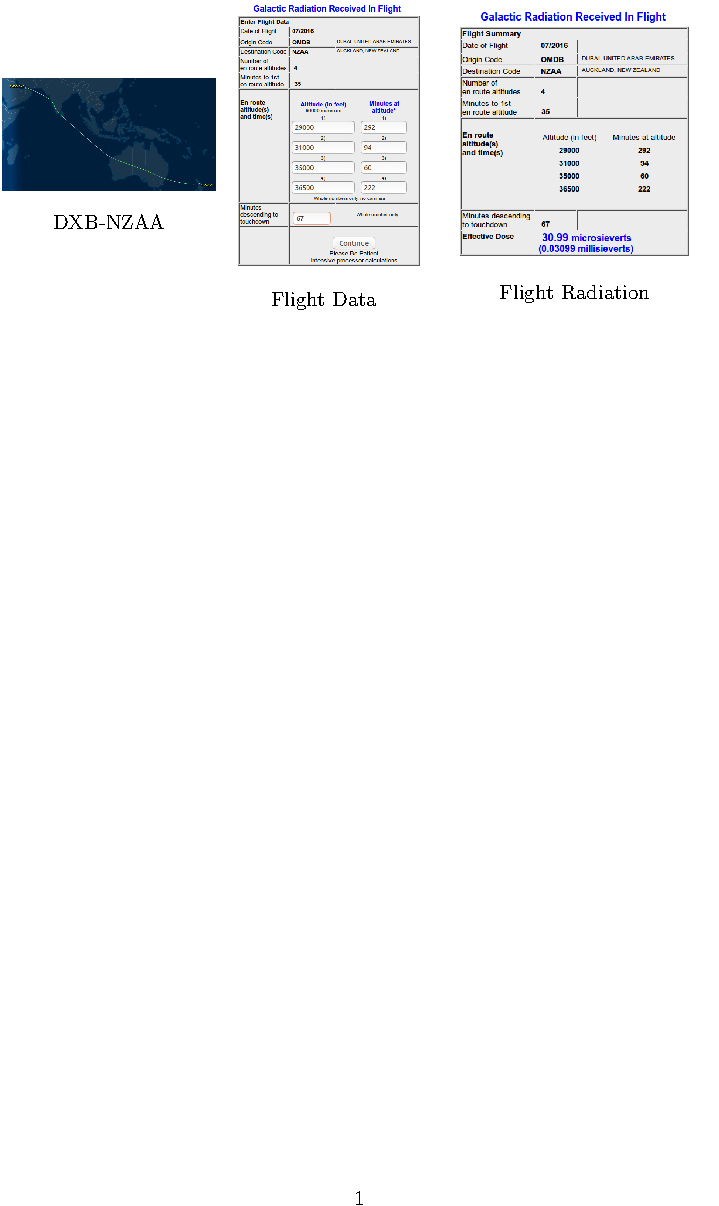
\includegraphics[scale=1.1]{images/DXB-TO-NZAA.pdf}   
 \end{figure}
 
\end{frame}
%\subsection{\semitransp[40]{REK-YYZ}}
\begin{frame}{REK-YYZ}

\begin{block}{REK-YYZ}
\end{block}
\begin{itemize}
\item Radiation Calculation

\end{itemize}
\vspace{-0.5cm}
\begin{figure}[]

   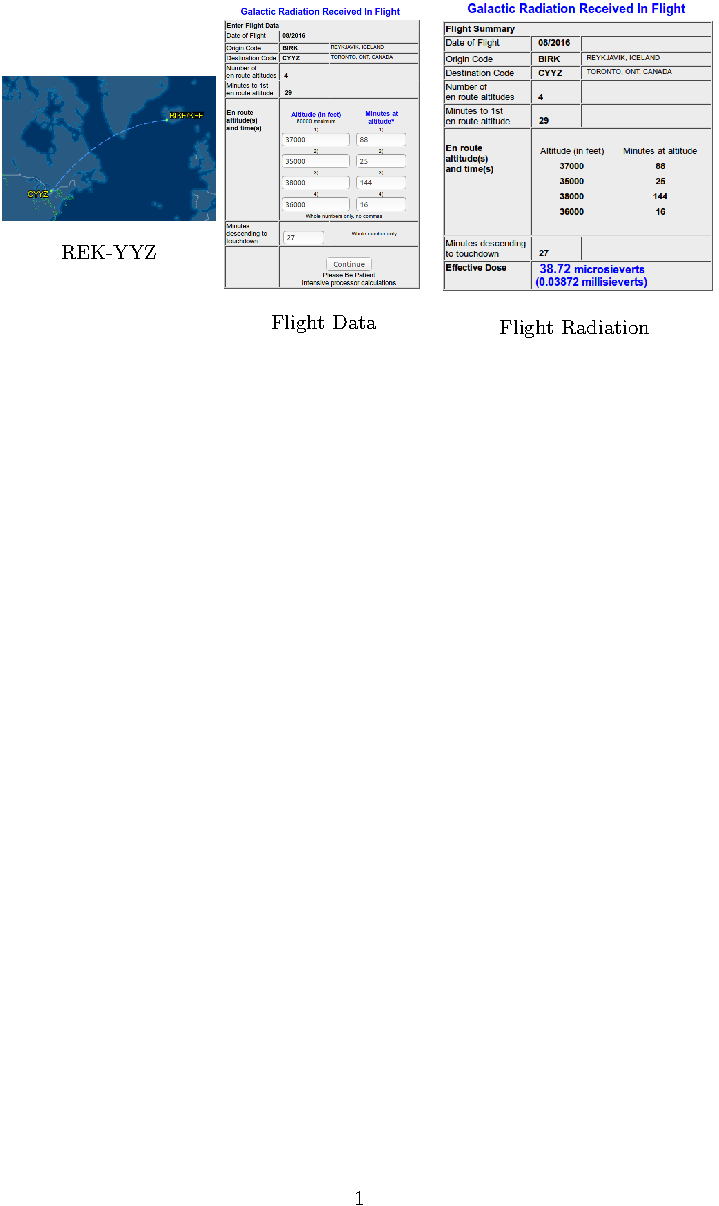
\includegraphics[scale=1.1]{images/REK-TO-YYZ.pdf}   
 \end{figure} 

\end{frame}




%\subsection{\semitransp[40]{DXB-KLAX}}
\begin{frame}{DXB-KLAX}

\begin{block}{DXB-KLAX}
\end{block}
\begin{itemize}
\item Radiation Calculation

\end{itemize}
\vspace{-0.5cm}
\begin{figure}[]

   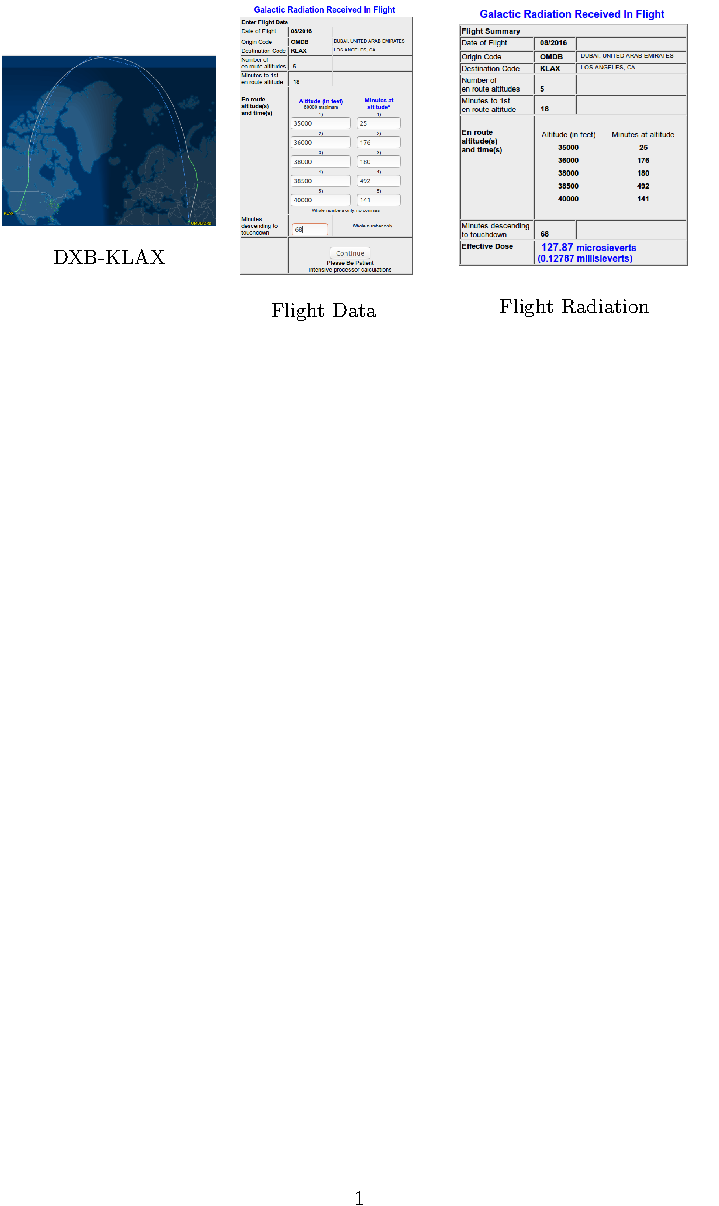
\includegraphics[scale=1.1]{images/DXB-TO-KLAX.pdf}   
 \end{figure} 
\end{frame}



\begin{frame}{PEK-KIAD}

\begin{block}{PEK-KIAD}
\end{block}
\begin{itemize}
\item Radiation Calculation

\end{itemize}
\vspace{-0.5cm}
\begin{figure}[]

   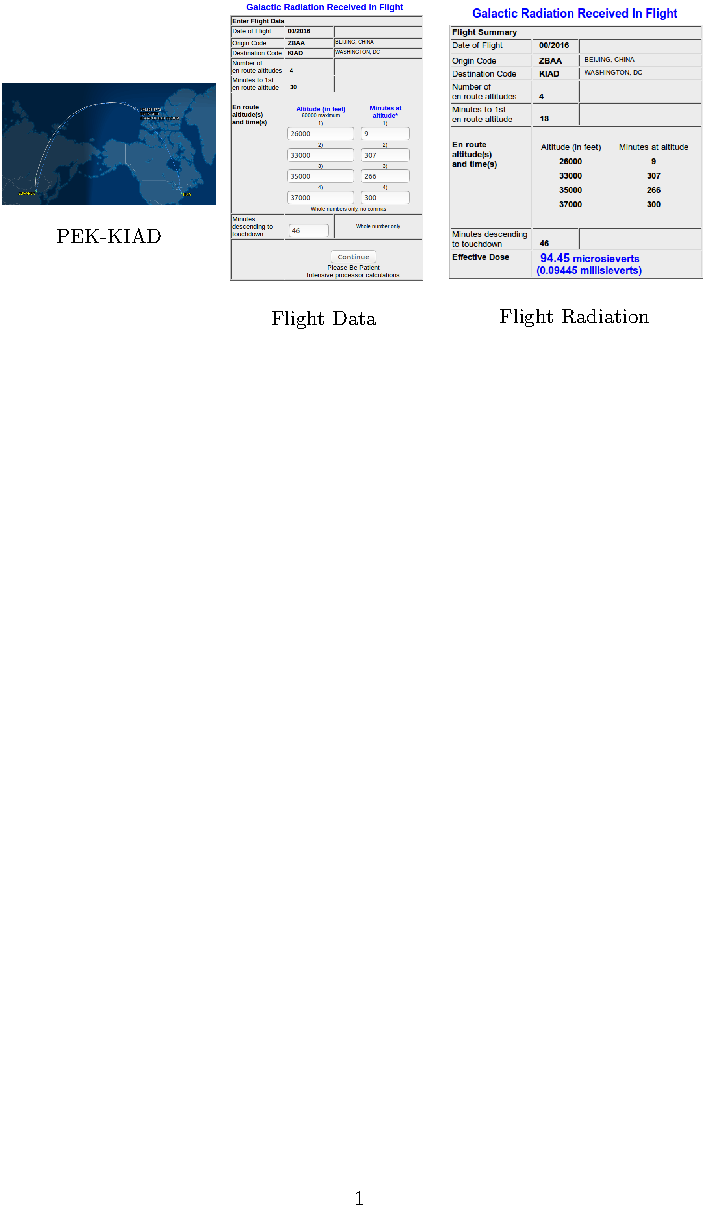
\includegraphics[scale=1.1]{images/PEK-TO-KIAD.pdf}   
 \end{figure} 
\end{frame}


%\subsection{\semitransp[40]{DXB-YYZ}}
\begin{frame}{DXB-YYZ}

\begin{block}{DXB-YYZ}
\end{block}
\begin{itemize}
\item Radiation Calculation

\end{itemize}
\vspace{-0.5cm}
\begin{figure}[]

   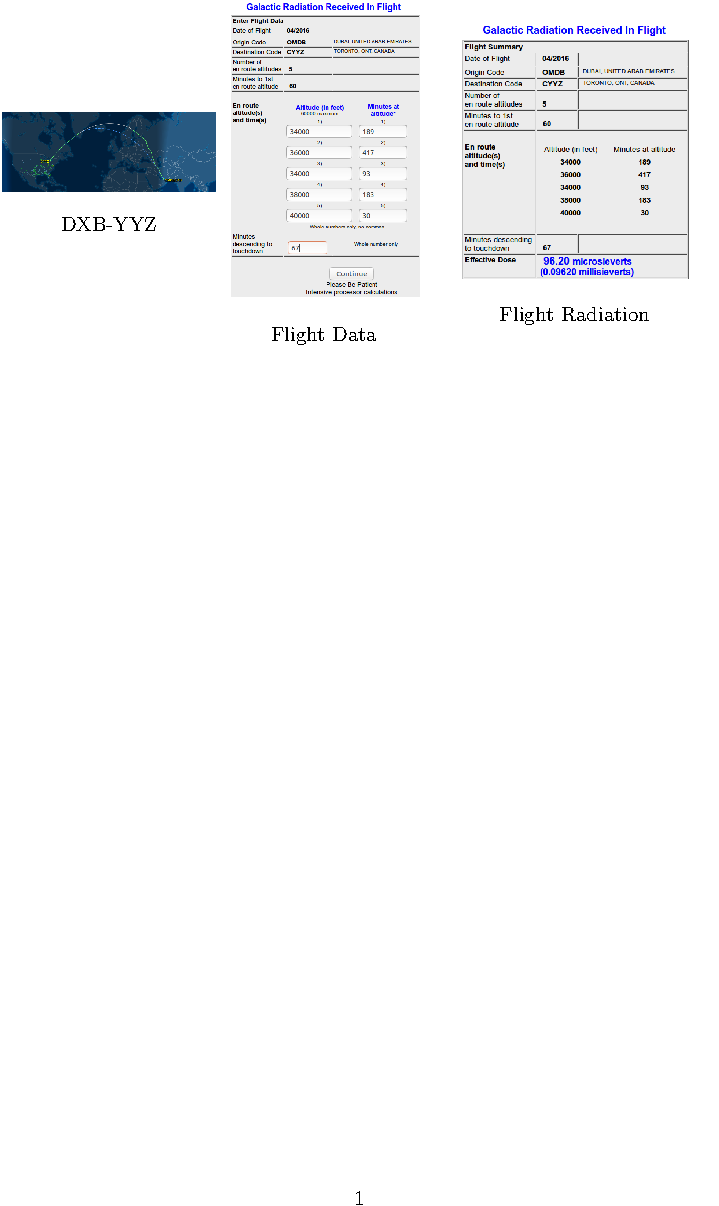
\includegraphics[scale=1.1]{images/DXB-TO-YYZ.pdf}   
 \end{figure} 
\end{frame}





\begin{frame}
\begin{block}{Summary}
\end{block}

\begin{table}[t]

\caption{Flight Radiation}
\scalebox{0.8}{

\begin{tabular}{ccccccc}
\toprule

              & Flight & Highest attitude & Minutes & Radiation  \\
              %& \multicolumn{1}{c}{resources} 
              % & \multicolumn{1}{c}{cache} 
                %& \multi%\subsection{\semitransp[40]{PEK-KIAD}}column{1}{c}{cache} 
               
               %  & \multicolumn{1}{c}{\color{red}{function}} 
                 
                 % & \multicolumn{1}{c}{\color{red}{generator}} \\
                \bottomrule   

 & DXB-NZAA    &  36500   & 222   &  30.99$msV$   \\ 
 & REK-YYZ    &  38000   & 144   &  38.99$msV$   \\
 & DXB-KLAX    &  40000   & 141   &  127.87$msV$   \\
 & PEK-KIAD    &  37000   & 300   &  94.45$msV$   \\
 & DXB-YYZ    &  40000  & 30  &  96.20$msV$   \\

\bottomrule
\end{tabular}
}

\end{table}
\end{frame}




\subsection{\semitransp[40]{EPCARD}}

\begin{frame}{EPCARD}
\begin{block}{EPCARD}

\begin{itemize}

\item EPCARD (European Program Package for the Calculation of Aviation Route Doses
\item It is based on the energy spectra of neutrons, protons, photons, electrons, positrons, muons, and pions
\item Input file format XML
\end{itemize}

\end{block}
\end{frame}

\begin{frame}{Flights}
\begin{block}{DXB-NZAA}

\begin{figure}[]

   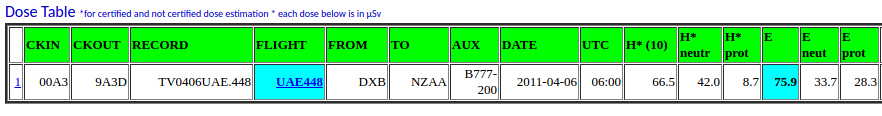
\includegraphics[width=1.0\textwidth]{EPCADR-RADIATION-DATA/OUTPUTS/DXB-NZAA.png}   
 \end{figure} 
 
\end{block}


\begin{block}{DXB-KLAX}

\begin{figure}[]

   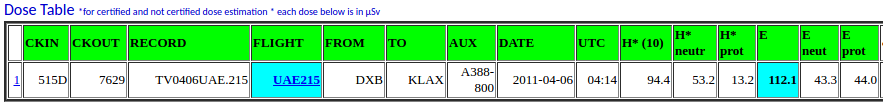
\includegraphics[width=1.0\textwidth]{EPCADR-RADIATION-DATA/OUTPUTS/DXB-KLAX.png}   
 \end{figure} 
 
\end{block}


\end{frame}



\begin{frame}{Flights}
\begin{block}{DXB-YYZ}

\begin{figure}[]

   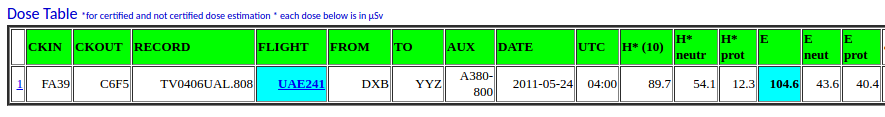
\includegraphics[width=1.0\textwidth]{EPCADR-RADIATION-DATA/OUTPUTS/DXB-YYZ.png}   
 \end{figure} 
 
\end{block}


\begin{block}{KEF-YYZ}

\begin{figure}[]

   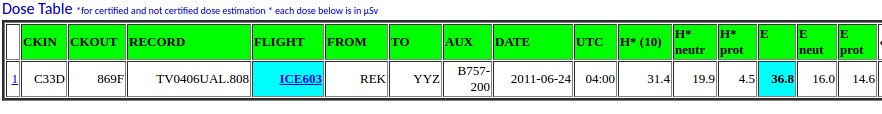
\includegraphics[width=1.0\textwidth]{EPCADR-RADIATION-DATA/OUTPUTS/KEF-YYZ.png}   
    
 \end{figure} 

\end{block}

\end{frame}



\begin{frame}
\begin{block}{Comparison}
\end{block}

\begin{table}[t]

\caption{Flight Radiation}
\scalebox{0.8}{

\begin{tabular}{ccccccc}
\toprule

              & Flight & CARI & EPCARD  \\
              %& \multicolumn{1}{c}{resources} 
              % & \multicolumn{1}{c}{cache} 
                %& \multi%\subsection{\semitransp[40]{PEK-KIAD}}column{1}{c}{cache} 
               
               %  & \multicolumn{1}{c}{\color{red}{function}} 
                 
                 % & \multicolumn{1}{c}{\color{red}{generator}} \\
                \bottomrule   

 & DXB-NZAA    &    30.99 $msV$ &  75.9  $msV$ \\ 
 & REK-YYZ     &    38.99 $msV$ & 36.8   $msV$ \\
 & DXB-KLAX    &    127.87 $msV$ &  112.1 $msV$ \\
 & PEK-KIAD    &    94.45 $msV$ &  77.7  $msV$\\
 & DXB-YYZ     &    96.20 $msV$ & 104.6  $msV$ \\

\bottomrule
\end{tabular}
}

\end{table}
\end{frame}


\section{Literature Review}

\subsection{\semitransp[40]{Literature Review}}

\begin{frame}
\begin{block} {Papers}

\end{block}
\end{frame}





























%
%\subsection{\semitransp[40]{Research Objectives}}
%\begin{frame}{Research Objectives}
%\vspace{-2.5cm}
%
%\begin{enumerate}CIVIL AEROSPACE MEDICAL INSTITUTE (CARI)
%%\newcommand{\labelenumii}{\Roman{enumii}}
%\setbeamertemplate{enumerate items}[default]
% \item The development of the probabilistic component --- randomized cache
% \item  Timing analysis for the probabilistic system
% \item Investigation of prediction effects for probabilistic systems under varying cache configuration
% \item  Predictable system on hardware with the help of probabilistic timing technique 
%\end{enumerate}
%
%
%%\begin{block}{(2) Technology Demonstration}
%%\begin{itemize}
%%\item Implementation of the aforementioned framework in an FPGA and integration with CubeSat 
%%\item ESA-Technology Readiness Level (4-6)~\cite{TRL}
%%\end{itemize}
%%
%%
%%
%%\end{block}
%\end{frame}
%
%\subsection{\semitransp[40]{Challenges}}
%\begin{frame}{Challenges}
%\vspace{-2.5cm}
%\begin{block}{Main Challenges}
%\end{block}
%\begin{itemize}
%\item Achieving randomization
%\item Applying probabilistic timing analysis
%\item Integration with processor
%\end{itemize}
%\end{frame}
%
%%%%%%%%%%%%%
%
%\subsection{\semitransp[40]{Timing Analysis}}
%%%%%%%%%%%%%
%
%\begin{frame}{Related Work/Background: Timing Analysis}
%
%
%
%\begin{block}{Deterministic Timing Analysis (DTA)}
%\end{block}
%\begin{itemize}
%\item Static Timing Analysis
%\item Measurement Timing Analysis
%\end{itemize}
%
%
%\vspace{0.2cm}
%\begin{block}{Probabilistic Timing Analysis (PTA)}
%\end{block}
%\begin{itemize}
%\item Measurement Based Probabilistic Timing Analysis
%\item Static Probabilistic Timing Analysis 
%
%\end{itemize}
%
%
%\begin{figure}[]
%
%   \includegraphics[scale=1]{images/timing-variants.pdf}
%   
%
%\end{figure}
%
%\end{frame}
%
%
%
%
%
%
%
%
%
%
%
%
%\begin{frame}{Related Work/Background: Deterministic Timing Analysis (DTA)}
%\vspace{-2cm}
%\begin{block}{Deterministic Timing Analysis}
%\end{block}
%
%\begin{itemize}
%%\item No platform required
%%\item Tight estimates  
%\item Mathematical representation of the code, and model of the platform
%\item Needs: Information about the HW/SW
%
%\item A possible limitation  --- the processor architecture itself
%%of the static
%%technique is the hardware (the processor architecture itself) because the processor hardware has
%%reached a level complexity that it is very hard to model
%\item E.g., Deterministic cache
%\end{itemize}
%\end{frame}
%
%%\begin{frame}{Related Work/Background: Deterministic Timing Analysis (DTA)}
%%\vspace{-1.5cm}
%%\begin{block}{Measurement based deterministic Timing Analysis}
%%\end{block}
%%\textcolor{red}{---Pros}
%%\begin{itemize}
%%\item Simpler to apply, platform needed
%%\item This technique is used to find the
%%execution times either on all execution paths, or on a subset of execution paths
%%\end{itemize}
%%
%%\textcolor{red}{---Cons}
%%
%%\begin{itemize}
%%\item It relies on observing the worst-case measured
%%execution time during the testing, and it is hard to execute it for all the test cases that might affect
%%the worst-case
%%\item Context dependent execution times may be missed 
%%
%%\end{itemize}
%%
%%\end{frame}
%
%\begin{frame}{Related Work/Background: Timing Analysis}
%\vspace{-0.2cm}
%\begin{block}{Probabilistic Timing Analysis}
%\end{block}
%\vspace{-0.3cm} 
%\begin{itemize}
%
%\item  Worst Case Execution Time estimations, to define bound with probability
%\item Multiple WCETs with an associated probability (probabilistic WCET or \small{p}WCET)
% \end{itemize}
%
%
%%\vspace{-0.5cm}
%\begin{figure}[]
%\centering
%%\caption{Timing Variants}
%  \captionsetup{justification=centering}  
%  %\input{./images/boxplottpdf}  
%  
%  %\vspace{-0.5cm}
% 
%   \includegraphics[scale=0.4]{images/pwcet.pdf}
%\end{figure}
%\end{frame}
%
%
%%\begin{frame}{Probabilistic Timing Analysis}
%%\begin{block}{Measurement-based PTA}
%%\end{block}
%%
%%
%%\begin{itemize}
%%
%%\item Complete runs of the program are made on the
%%time-randomized target platform
%%\item All potential execution times must have a probability of being
%%exercised
%%\item From this and sufficiently large number of i.i.d observations
%%(in the order of hundreds) we can use EVT to derive pWCET
%%estimations
%%
%%\end{itemize}
%%
%%
%%
%%\end{frame}
%
%
%
%
%
%
%
%
%\section{Related Work/Background}
%\subsection{\semitransp[40]{Time-Predictable Architecture}}
%%%%%%%%%%%%%
%\begin{frame}{Related Work/Background: Time Predictable Architecture}
%%%\begin{block}{Deterministic Approach}
%%\end{block}
%\large{\textbf{\color{polymtlred}{Deterministic Approach:}}}
%
%%\vspace{0.2cm}
%
%%\begin{itemize}
%%\vspace{-0.4cm}
%%\item Unpredictable timing behaviour 
%%\item Probabilistic approach
%%\end{itemize}
%\begin{block}{Komodo~\cite{kreuzinger1999komodo}}
%\end{block}
%\begin{itemize}
%\vspace{-0.4cm}
%\item Used to execute Java application
%\item Access memory at higher clock frequency than for the pipeline 
%\end{itemize}
%
%\begin{block}{Java Optimized Processor~\cite{schoeberl2009time}}
%\end{block}
%\begin{itemize}
%\vspace{-0.4cm}
%\item Time Predictable Java Processor
%\item WCET analysis at Java bytecode
%\end{itemize}
%
%
%\begin{block}{MERASA~\cite{ungerer2010merasa}}
%\end{block}
%\begin{itemize}
%\vspace{-0.4cm}
%\item Multicore processor
%\item Used DTA for WCET 
%\end{itemize}
%
%
%\end{frame}
%
%\subsection{\semitransp[40]{Probabilistic Systems/Components}}
%%%%%%%%%%%%%
%\begin{frame}{Related Work/Background: Probabilistic Systems/Components}
%
%\large{\textbf{\color{polymtlred}{Probabilistic Approach:}}}
%%\begin{itemize}
%%\item Probabilistic modeling is in close match with actual nature
%%of the system
%%\item Chances for missing the deadline is probabilistically arguable, e.g. $10^{-6}$, $10^{-12}$, etc
%%\item The system as a whole has a distinct prob. of failure
%%\end{itemize}
%%\offslide<1->
%%\begin{figure}
%% \includegraphics[scale=0.1]{images/ps.png}
%%\end{figure}
%
%
%
%
%
%
%\begin{block}{Probabilistically Analyzable Cache~\cite{kosmidis2013cache}}
%\end{block}
%\begin{itemize}
%\item Time-randomization concept 
%\item Deterministic placement and replacement make it impossible to drive true probabilities for different execution-time processor, and communication 
%\item Simulated work
%\item Used EVT for MBPTA
%\end{itemize}
%
%
%
%
%\begin{block}{Probabilistically Analyzable Bus~\cite{Jalle:2014:BDT:2616606.2616668}}
%\end{block}
%\begin{itemize}
%\item Bus Designs for Time-probabilistic Multicore Processors
%
%\item Randomized arbitration
%\end{itemize}
%
%
%\end{frame}
%
%
%
%
%
%\section{Contribution}
%%%%%%%%%%%%%
%\begin{frame}{Contribution}
%%\begin{block}{\textbf{(1) Probabilistically Analyzable Time-Predictable Architecture}}
%%{Definition, Modification, and Implementation}
%%\end{block}
%\vspace{-2cm}
%\begin{block}{\onslide<1->{\textbf{A Probabilistically Analyzable Cache Implementation on FPGA~\cite{anwar2015probabilistically} }}}
%\onslide<2->{MBPTA, WCET Estimation}
%\end{block}
%\begin{block}{\onslide<3->{\textbf{A Probabilistically Analyzable Cache to Improve Timing Analysis Bound}}}
%\onslide<4->{SPTA, MBPTA, WCET Estimation, LRU}
%\end{block}
%%\begin{block}{\onslide<4->\textbf{(4) Probabilistic Multi-core Architecture}}
%%{Bus design, Last Level Cache (LLC)}
%%\end{block}
%\end{frame}
%
%%\subsection{\semitransp[40]{(1) Time-Predictable Architecture}}
%%%%%%%%%%%%%%
%%\begin{frame}{Time Predictability}
%%\begin{block}{Novel Computer Architecture}
%%
%%Need to modify architectural components/features of a current processor.
%%\vspace{0.2cm}
%%\begin{itemize}
%%\item  Pipelines will be simple, with minimum dependencies between instructions
%%
%%\item  \textit{Randomized cache}, which helps to drive tighter WCET analysis
%%
%%\item  Avoid processor's out-of-order execution as it increases WCET complexity
%%
%%\item  In-order to avoid an unbounded timing effect, time-predictable processor uses prefetch queue and double buffer
%%
%%\item Use static branch prediction instead of dynamic predictors
%%
%%\item Chip multi-processor with one thread per processor 
%%
%%\item Randomized Time Division Multiplexing Access (TDMA) arbiter
%%
%%\end{itemize}
%%\end{block}
%%\end{frame}
%
%
%\subsection{\semitransp[40]{A Probabilistically Analyzable Cache Implementation on FPGA}}
%\subsection{\semitransp[40]{Cache Design Consideration to Improve Timing Analysis Bounds}}
%
%
%
%%%%%%%%%%%%%%%%%%%%%%%%%%%%%%%%%%%%%%%%%%%%%%%%%
%%\section{A Probabilistically Analyzable Cache Implementation on FPGA}
%%%%%%%%%%%%%
%\begin{frame}{Contribution}
%\vspace{-1.2cm}
%\begin{block}{A Probabilistically Analyzable Cache Implementation on FPGA}
%\end{block}
%\begin{columns}
%\column{.4\textwidth}
%\begin{itemize}
%
%%\item  Implementation of a probabilistically Analyzable instruction and data cache for Ion MIPS32 processor
%\item  Probabilistic cache
%\item  ION MIPS-32 processor
%\item  Random number generator 
%%for a real-time program without knowing the detailed knowledge of hardware model
%\item Parametric hash function
%
%\end{itemize}
%\column{.70\textwidth}
%\begin{figure}
% %\centering
%  %%\captionsetup{justification=centering}
%      \begin{flushright}
%      
%     %\hspace{3cm} 
%   \includegraphics[scale=0.70]{images/cache_structure_c.pdf}
%  %\caption{Structure of the proposed cache.}
%    \end{flushright}
%    
%
%\end{figure}
%
%\end{columns}
%\end{frame}
%
%\begin{frame}{A Probabilistically Analyzable Cache Implementation on FPGA}
%\begin{block}{Parametric Hash Function}
%\end{block}
%\begin{columns}
%
%\column{.5\textwidth}
%
%\vspace{-4cm}
%\begin{itemize}
%\item Proposed by~\cite{Cazorla:2013:PPA:2465787.2465796}
%\item Deterministic placement--- no probability
%\item Used to randomized the cache placement
%
%%\item Placement is randomized
%%\item Barrel shifter  used to rotate the address bits 
%
%\end{itemize}
%
%
%
%\column{.9\textwidth}
%\begin{figure}
% 
%  \hspace{-4.5cm}   
%   \includegraphics[scale=0.8]{images/hash.pdf}
%%   \caption{Hash Function}
%\label{fig:hash}
%\end{figure}
%\end{columns}
%\end{frame}
%
%\begin{frame}{A Probabilistically Analyzable Cache Implementation on FPGA}
%\vspace{-1.5cm}
%\begin{block}{Cache Design}
%\end{block}
%
%%\begin{columns}
%
%
%%\column{.6\textwidth}
%%\vspace{-5cm}
%\begin{itemize}
%\item  The model is developed in VHDL
%\item  Configurable Parameters --- \textit{cache line size, cache size, associativity, replacement policy}, and \textit{write policy}
%\item Placement policy --- Random placement and modulo placement
%\item  Replacement policy --- Random replacement and LRU
%\item  For data write it supports \textit{write-through} and \textit{write-back} policies
%\item  For cache miss it supports \textit{write-allocate} and \textit{no write-allocate}
%\item Cache Generator for FPGAs~\cite{yiannacouras2003parameterized}
%\end{itemize}
%
%%\column{.5\textwidth}
%%
%%\vspace{-0.5cm}
%%\begin{figure}
%%
%%\vspace{0.1cm}
%%       \includegraphics[scale=0.7]{images/vhdlbasic.pdf}
%%   
%%\end{figure}
%%\end{columns}
%
%
%\end{frame}
%
%
%
%%
%%\begin{frame}{A Probabilistically Analyzable Cache Implementation on FPGA}
%%\begin{block}{Hardware Implementation}
%%\end{block}
%%
%%%\begin{columns}
%%%
%%%
%%%\column{.5\textwidth}
%%
%%\begin{itemize}
%%\item A random placement policy used a parametric hash function
%%\item A random replacement policy used high quality random number
%%\item Pseudo random number (MT19937)
%%\item ION Core
%%
%%\end{itemize}
%%
%%\vspace{-1.5cm}
%%
%%%\column{.7\textwidth}
%%
%%
%%%
%%%\end{columns}
%%\end{frame}
%
%
%
%
%
%\begin{frame}{Measurement Based Probabilistic Timing Analysis}
%%
%\vspace{-3cm}
%\begin{block}{What is Extreme Value Theory}
%\end{block}
%
%\begin{itemize}
%
%
%\item Used to model the smallest or largest value among a large set of independent, identically distributed random values representing measurements or observations
%\item The \small{p}WCET estimate is obtained by applying Extreme
%Value Theory
%
%%\item Reduce the cost of acquiring the knowledge needed for computing trustworthy WCET bounds
%%\item Extreme value theory is used to find the probability of rare events
%%\item EVT provides an estimation for the maximum of a sequence of i.i.d random variable
%%\item The timing values should be regarded as random variables that must have i.i.d property
%%\item Properties checked through statistical tests
%\end{itemize}
%%\begin{figure}
%%\includegraphics[scale=0.49]{images/evt.png}
%%\end{figure}
%
%\end{frame}
%
%\begin{frame}{Measurement Based Probabilistic Timing Analysis}
%
%
%\begin{block}{Applying Extreme Value Theory}
%\end{block}
%\vspace{-0.3cm}
%\begin{itemize}
%\item Collect timing measurements (execution times)
%\item Independent and Identical Distributed (i.i.d)
%%\item Properties checked through statistical tests
%\item \textit{Kolmogorov-Smirnov} test --- identically distribtuted (Threshold - 0.05)
%\item \textit{Wald-Wolfowitz} --- independence test ($<1.96$)
%%\item Modeled the data with Gumbel distribution ($\sigma$ and $\mu$)
%%\item Utilization of EVT to \small{p}WCET estimating
%
%
%\end{itemize}
%
%\begin{figure}
%\vspace{-0.3cm} 
%
%       \includegraphics[width=0.50\textwidth]{images/gumbel.png}
%    
%\end{figure}
%
%\end{frame}
%
%
%
%
%
%
%
%\begin{frame}{A Probabilistically Analyzable Cache Implementation on FPGA}
%
%\begin{block}{Experimental Setup}
%\end{block}
%
%\begin{itemize}
%\item Xilinx ML505 FPGA board
%\item 4-KB cache memories for data and instructions
%\item  M\"alardalen benchmarks \cite{mrtc:bench}
%\item Drived execution time profile using MBPTA with 1000 runs per profile
%\item Resource utilization and overhead
%\end{itemize}
%
%\begin{table}[t]
%
%\caption{Resource Utilization and Overhead (Virtex-5)}
%\scalebox{0.8}{
%
%\begin{tabular}{ccccccc}
%\toprule
%
%              & Available & Deterministic & Probabilistic & \color{red}{Hash} & \color{red}{Random} & Overhead (\%) \\
%              & \multicolumn{1}{c}{resources} 
%               & \multicolumn{1}{c}{cache} 
%                & \multicolumn{1}{c}{cache} 
%                 & \multicolumn{1}{c}{\color{red}{function}} 
%                  & \multicolumn{1}{c}{\color{red}{generator}} \\
%                \bottomrule   
%%\cmidrule(lr){3-5}
%%              &   &  Cache & Hash	& MT19937 &  \\
%%\midrule
%%%Available     & 69120    &       69120   & 69120       
%%LUT Flip Flop  & 1904    &  1792   &  656   &  117  & 34.7    \\
%LUT Flip Flop  & 17708    &  1904   & 1792    &  656  & 117 & 4.36\% \\ 
%Slice LUTs     & 69120    &   6026  &   5637  &  660  &419 & 1.56 \%  \\
%%%BRAMs          & 4       &  6      &  2     &  1    & 225\%\\
%\bottomrule
%\end{tabular}
%}
%
%\end{table}
%
%\end{frame}
%
%\begin{frame}{A Probabilistically Analyzable Cache Implementation on FPGA}
%\vspace{-1.5cm}
%\begin{block}{Experimental Results}
%\end{block}
%%\vspace{2cm}
%%\begin{columns}
%%
%%\column{.7\textwidth}
%%\vspace{-4cm}
%%\vspace{-2cm}
%\begin{itemize}
%%\vspace{-2cm}
%\item Direct mapped to set-associative cache 
%\item WCET improvement: \\ --- 11\% for 2-way SA \\ --- 8\% for 4-way SA \\ --- 6\% to 8-way SA
%\item 5-15\% improvement for \small{p}WCET
%\item Random replacement has a lower probability of cache conflicts 
%\item Probabilistic cache
%provide best hardware platform to PTA techniques to \\ estimate pWCET
%with less pessimism 
%\end{itemize}
%%\hspace{-5cm}
%%\column{.5\textwidth}
%
%%\begin{figure}
%%\hspace{-2cm}
%%       \includegraphics[scale=0.4]{images/boxplot.pdf}
%%       \caption{Execution Time Measurements}
%%
%%\end{figure}
%%\end{columns}
%\end{frame}
%
%
%
%
%
%
%\begin{frame}{A Probabilistically Analyzable Cache Implementation on FPGA}
%\begin{block}{Experimental Results}
%\end{block}
%\begin{table}[tb]
%  \caption{Predicted pWCET ($T_p$) at $10^{-3}$ exceedance probability versus measured WCET ($T_m$) for the RND cache. Times are shown in milliseconds.}
%\label{pWCETTiming}
%\begin{tabular}{lllllllll}
%\toprule
%Benchmark & \multicolumn{2}{l}{Direct} & \multicolumn{2}{l}{2-way} & \multicolumn{2}{l}{4-way} & \multicolumn{2}{l}{8-way}    \\
%\cmidrule(lr){2-3} \cmidrule(lr){4-5} \cmidrule(lr){6-7} \cmidrule(lr){8-9}  
%                &  $T_m$ & $T_p$  &  $T_m$ & $T_p$ &  $T_m$ & $T_p$ &  $T_m$ & $T_p$ \\
%\midrule
%
%
%cnt       & \color{red}{11.58} & \color{red}15.35  & 8.30 & 9.76 & 7.11 & 8.75& \color{red}6.52 & \color{red}7.90    \\ 
%
%bs        &  3.77  & 6.10   & 3.42 & 5.06  & 3.17 & 4.22 & 2.75 & 3.77 \\ 
%fac &  6.67  & 9.31  & 5.44 & 7.42 & 4.62 & 6.36 & 3.33 & 3.95 \\ 
%crc       &  \color{red}{4.49}  & \color{red}{7.23}  & 2.50 & 5.06  & 2.77 & 4.90  & \color{red}{2.82} & \color{red}{4.29}\\ 
%qsort-exam     &  9.98  & 12.08  & 9.10 & 11.18 & 7.83 & 10.26 & 6.43 & 8.34 \\ 
%select    &  3.80  & 5.43  & 2.98 & 4.55  & 2.59 & 3.44  & 2.22 & 3.02  \\ 
%\bottomrule
%\end{tabular}
%\end{table}
%
%%\begin{figure}[t!]
%%
%% \centering
%%  \captionsetup{justification=centering}  
%%  %\input{./images/boxplot.pdf}  
%%   \includegraphics[scale=0.79]{images/boxplot.pdf}
%%   \caption{Execution Time Measurement}
%%\label{fig:boxplot}
%%\end{figure}
%
%\end{frame}
%
%
%\begin{frame}{A Probabilistically Analyzable Cache Implementation on FPGA}
%\begin{block}{Comparison}
%\end{block}
%
%\begin{table}[]
%\caption{Deterministic/Probabilistic WCETs and respective bounds}
%%\label{percentage difference}
%%\hspace{2.8cm} 
%\scalebox{0.8}{
%\centering
%\begin{tabular}{lcccccccc}
%\toprule
%Benchmark & \multicolumn{8}{c}{Execution-Time (ms)}    \\
%\cmidrule(lr){2-2} \cmidrule(lr){4-4} \cmidrule(lr){6-6} \cmidrule(lr){8-8} 
%
%& Deterministic  & & Prediction  & & Probabilistic & & Prediction \\
% &  \multicolumn{1}{l}{\hspace{0.5cm}{Cache (WCET)}} & & bound & & Cache (WCET) & & bound\\
%  
% 
%
%  \midrule
%
% 
%
%%  \midrule
%%
%%
%cnt       &   \multicolumn{2}{c}{5.04} & \multicolumn{2}{c}{10.33}    & \multicolumn{2}{c}{6.52} & \multicolumn{1}{c}{7.90} & \\
%bs       &   \multicolumn{2}{c}{2.57} & \multicolumn{2}{c}{6.77}    & \multicolumn{2}{c}{2.75} & \multicolumn{1}{c}{3.77} \\
%fac       &   \multicolumn{2}{c}{2.93} & \multicolumn{2}{c}{5.45}    & \multicolumn{2}{c}{3.33} & \multicolumn{1}{c}{3.95}\\
%crc       &   \multicolumn{2}{c}{2.50} & \multicolumn{2}{c}{6.13}    & \multicolumn{2}{c}{2.82} & \multicolumn{1}{c}{4.29} \\
%qsort-exam       &   \multicolumn{2}{c}{5.43} & \multicolumn{2}{c}{11.09}    & \multicolumn{2}{c}{6.43} & \multicolumn{1}{c}{8.34} \\
%select       &   \multicolumn{2}{c}{3.91} & \multicolumn{2}{c}{5.34}    & \multicolumn{2}{c}{4.12} & \multicolumn{1}{c}{5.18}
%\\
%\bottomrule
%\end{tabular}
%}
%\end{table}
%
%\end{frame}
%
%\begin{frame}{A Probabilistically Analyzable Cache Implementation on FPGA}
%\begin{block}{Comparison}
%\end{block}
%
%
%
%\begin{table}[h]
%\caption{Pessimism between predicted pWCETs at $10^{-3}$ exceedance probability versus deterministic cache}
%\scalebox{0.70}{
%\centering
%\begin{tabular}{lcccccc}
%\toprule
% & \multicolumn{6}{c}{Pessimism Difference(\%)}   \\
%\cmidrule(lr){2-2} \cmidrule(lr){3-3} \cmidrule(lr){2-2} \cmidrule(lr){4-4}\cmidrule(lr){5-5} \cmidrule(lr){6-6} \cmidrule(lr){7-7}
%
%
%  
% & cnt     & bs   & fac  & crc &  qsort &  select  \\
%
%
%  \midrule
%
%Deterministic cache       &   \multicolumn{1}{c}{68.83} &
%
% \multicolumn{1}{c}{89.93}  & \multicolumn{1}{c}{60.14}&\multicolumn{1}{c}{84.12}
%  &   \multicolumn{1}{c}{68.52} &   \multicolumn{1}{c}{30.91}   \\
% 
%Probabilistic cache       &   \multicolumn{1}{c}{19.14} &
%
% \multicolumn{1}{c}{31.28}  & \multicolumn{1}{c}{17.033}&\multicolumn{1}{c}{41.35}
%  &   \multicolumn{1}{c}{25.86} &   \multicolumn{1}{c}{22.79}   \\
%
%
%\bottomrule
%\end{tabular}
%}
%\end{table}
%
%\begin{figure}
%
%       \includegraphics[width=0.68\textwidth]{images/tpc-example.pdf}
%       \end{figure}
%
%
%\end{frame}
%
%
%
%
%
%
%
%
%%\begin{frame}{A Probabilistically Analyzable Cache Implementation on FPGA}
%%\vspace{-1.5cm}
%%\begin{block}{Experimental Results}
%%\end{block}
%%
%%\begin{itemize}
%%\item MBPTA is used to find the probability of rare events
%%\item MBPTA is used to predict the worst case execution time of the applications running on the
%%processor
%%\item The timing values should be regarded as random variables that must have i.i.d property
%%\item Properties checked through statistical tests
%%\item \textit{Kolmogorov-Smirnov} test --- identically distribtuted (Threshold-0.05)
%%\item \textit{Wald-Wolfowitz} --- independence test $(< 1.96)$
%%\end{itemize}
%%\end{frame}
%
%
%\begin{frame}{A Probabilistically Analyzable Cache Implementation on FPGA}
%\vspace{-3.5cm}
%\begin{block}{Summary}
%\end{block}
%
%\begin{itemize}
%
%\item Random cache implementation can successully provide a probabilistically analyzable cache  
%
%\item MBPTA can be applied to provide safe bounds with arbitrary accuracy
%
%\end{itemize}
%\end{frame}
%
%
%
%
%
%
%
%
%
%
%
%
%
%
%
%%%%%%%%%%%%%
%
%
%
%
%
%
%
%
%
%
%\begin{frame}{Contribution}
%\vspace{-2.3cm}
%\begin{block}{Cache Design Consideration to Improve Timing Analysis Bounds}
%\end{block}
%\begin{itemize}
%\item  Time Prediction under  varying cache parameters (associativity, cache size, and line size)
%\item  MBPTA and SPTA
%\item  Predictibility with cache enabled with deterministic approach, e.g. LRU
%\item  The exceedance threshold set to $10^{-03}$
%\end{itemize}
%
%\end{frame}
%
%
%
%
%\begin{frame}{Cache Design Consideration to Improve Timing Analysis Bounds}
%\vspace{-2.3cm}
%\begin{block}{Experimental Setup}
%\end{block}
%\begin{itemize}
%\item  Leon-3 Processor
%\item  gcc 4.8.4 with no optimization of binary code
%\item SPTA method is applied on the address traces
%\item MBPTA based EVT
%\item SPTA based on Markov Chain
%\item WCET estimates for the deterministic hardware, e.g. LRU
%\end{itemize}
%
%\end{frame}
%
%
%
%
%
%\begin{frame}{Cache Design Consideration to Improve Timing Analysis Bounds}
%
%\vspace{-2.3cm}
%\begin{block}{Experimental Evaluation}
%\end{block}
%\begin{itemize}
%%\item Study the influence of \textit{associativity,cache size,} and \textit{line size} on the WCET estimates for the time-prediction
%\item  Prediction analysis under Associativity 
%\item  Prediction analysis under Cache Size
%\item  Prediction analysis under Line Size
%\item Evaluated by MBPTA and SPTA
%\end{itemize}
%
%\end{frame}
%
%
%
%%
%%\begin{frame}{Cache Design Consideration to Improve Timing Analysis Bound}
%%\vspace{-1.7cm}
%%\begin{block}{Static PTA}
%%\end{block}
%%\begin{itemize}
%%
%%\item The SPTA method used in this work is based on the Markov chains. 
%%%\item  Applied
%%%to a set associative cache 
%%%\item The method uses a memory trace as the input, and computes a pWCET as
%%%the output
%%\item It poses a property that the probability distribution of the future state
%%of a system depends only on the current state
%%\item The current
%%state explains the status of the system, and the transition matrix describes how the system transits
%%into the future state
%%
%%\end{itemize}
%%\end{frame}
%
%
%\begin{frame}{Cache Design Consideration to Improve Timing Analysis Bounds}
%\vspace{-0.2cm}
%\begin{block}{Prediction Analysis under Associativity---MBPTA}
%\end{block}
%\vspace{-0.38cm}
%\begin{itemize}
%%\item  Three Set-Associative (SA) cache structures --- SA-2, SA-4, and SA-8
%%\item  Execution Time Improvement
%%\item  Higher the Associativity, smaller the overestimation
%\item  The time prediction is varied between 5.09 \% to 3.11 \% for SA-2, this pessimism is decreased  from 4.26 \% to 1.33 \%  for SA-8
%\end{itemize}
%
%
%\vspace{-0.2cm}
%\begin{figure}
% \centering
%  \captionsetup{justification=centering}    
%   \includegraphics[width=0.85\textwidth]{images/mbpta.pdf}
%\end{figure}
%
%
%\end{frame}
%
%
%
%
%\begin{frame}{Cache Design Consideration to Improve Timing Analysis Bounds}
%\vspace{-0.2cm}
%\begin{block}{Prediction Analysis under Associativity---SPTA}
%\end{block}
%\vspace{-0.38cm}
%\begin{itemize}
%%\item  SPTA applied on the address traces of the code
%%\item  As not predictable as for MBPTA
%%\item  Higher the Associativity, smaller the overestimation
%%\item  The pessimism does not decrease at higher cache associativity
%\item The average difference between the predicted time and the maximum execution time for SPTA is 3.07 \% and 1.77\% for MBPTA
%\end{itemize}
%
%
%\vspace{-0.1cm}
%\begin{figure}
%    
%   \includegraphics[width=0.74\textwidth]{images/spta.pdf}
%\end{figure}
%
%
%\end{frame}
%
%
%\begin{frame}{Cache Design Consideration to Improve Timing Analysis Bounds}
%\vspace{-0.2cm}
%\begin{block}{Prediction Analysis under Cache Size---MBPTA}
%\end{block}
%\vspace{-0.38cm}
%\begin{itemize}
%%\item  Study the effects of the cache size on time prediction
%%\item  The prediction difference the predicted time and the maximum execution time is decreased by increasing the cache size
%%\item The level of pessimism is decreased from 5.01 \% to 0.43 \%
%\item Increasing the cache size helps to fit the binary code size into the cache and this ultimately improves the cache hit ratio
%\end{itemize}
%
%
%\vspace{-0.1cm}
%\begin{figure}
% \centering
%  \captionsetup{justification=centering}    
%   \includegraphics[width=0.74\textwidth]{images/cachesize-mbpta.pdf}
%\end{figure}
%\end{frame}
%
%
%
%\begin{frame}{Cache Design Consideration to Improve Timing Analysis Bounds}
%\vspace{-0.3cm}
%\begin{block}{Prediction Analysis under Cache Size---SPTA}
%\end{block}
%\vspace{-0.3cm}
%\begin{itemize}
%%%\item  The pessimism observed under the SPTA is in between 1.25 \% to 3.53 \%
%\item  The average pessimistic difference between the predicted time and the actual execution time
%from 2-kB to 8-kB is 2.38\%. Whereas, for MBPTA, this difference factor is reduced to 1.93\%. 
%%SPTA pessimistic nature does not help to minimize the level of pessimism as much MBPTA does
%\end{itemize}
%
%
%\vspace{-0.1cm}
%\begin{figure}
% \centering
%  \captionsetup{justification=centering}    
%   \includegraphics[width=0.69\textwidth]{images/cachesize-spta.pdf}
%\end{figure}
%
%
%\end{frame}
%
%\begin{frame}{Cache Design Consideration to Improve Timing Analysis Bounds}
%\vspace{-0.25cm}
%\begin{block}{Prediction Analysis under Line Size---MBPTA}
%\end{block}
%\vspace{-0.3cm}
%\begin{itemize}
%%\item  Used two cache lines, i.e 16-bytes and 32-bytes line size, Associativity-4 and the capacity is 4-KB
%\item  Increase in the line size decrease the \small{p}WCET estimates. Because larger cache lines minimize the number of loads from the memory that help to reduce the pessimisim.
%%\item The average reduction in predicted time is 1.87 \%
%\end{itemize}
%
%
%\vspace{-0.1cm}
%\begin{figure}
% \centering
%  \captionsetup{justification=centering}    
%   \includegraphics[width=0.74\textwidth]{images/cacheline-mbpta.pdf}
%\end{figure}
%
%
%\end{frame}
%
%
%
%\begin{frame}{Cache Design Consideration to Improve Timing Analysis Bounds}
%\vspace{-0.2cm}
%\begin{block}{Prediction Analysis under Line Size---SPTA}
%\end{block}
%\vspace{-0.34cm}
%\begin{itemize}
%\item  Prediction improves as compare with associativity and cache sizes
%%\item  Example: \textit{Ud} the level of pessimism goes from 16.39 \% to 6.14 \%
%\end{itemize}
%
%
%\vspace{-0.3cm}
%\begin{figure}
% \centering
%  \captionsetup{justification=centering}    
%   \includegraphics[width=0.82\textwidth]{images/cacheline-spta.pdf}
%\end{figure}
%
%
%\end{frame}
%
%
%\begin{frame}{Cache Design Consideration to Improve Timing Analysis Bounds}
%\vspace{-1cm}
%\begin{block}{Comparison}
%\end{block}
%
%\vspace{-0.7cm}
%
%\begin{table}[]
%\centering
%
%\caption*{Level of Pessimism Introduced by varying Cache Parameters}
%%\vspace{-0.7cm}
%%\hspace*{-2.3em}
%\scalebox{0.8}{
%\centering
%\begin{tabular}{lcccccccccccccc}
%\toprule
%Benchmark & \multicolumn{12}{c}{Level of Pessimism(\%)}   \\
%\cmidrule(lr){2-3} \cmidrule(lr){4-5} \cmidrule(lr){6-7} \cmidrule(lr){8-9}\cmidrule(lr){10-11}\cmidrule(lr){12-13}\cmidrule(lr){14-15}
%
%
%  
%  & Associativity      && Associativity && Size &&Size &&Line size && Line size && \\
%& \multicolumn{1}{l}{SA-2 to SA-8} &&{SA-2 to SA-8} &&SA 2-8 kB &&SA 2-8 kB && SA 16-32 B && SA 16-32 B && \\ 
%& \multicolumn {1}{l}{MBPTA} &&SPTA &&MBPTA &&SPTA&&MBPTA &&SPTA && \\
%  \midrule
%
%
%
%
% 
%ud       &   \multicolumn{2}{c}{4.26} & \multicolumn{2}{c}{3.96} & 
%\multicolumn{2}{c}{2.27} & \multicolumn{2}{c}{2.26} 
%& \multicolumn{2}{c}{2.43} & \multicolumn{2}{c}{2.37}
%
%
%  \\ 
%cover    &   \multicolumn{2}{c}{1.24} & \multicolumn{2}{c}{1.23} &
%\multicolumn{2}{c}{1.13} & \multicolumn{2}{c}{1.41} 
%& \multicolumn{2}{c}{0.45}
%& \multicolumn{2}{c}{0.52}
%\\
%
%expint &   \multicolumn{2}{c}{\color{red}{0.95}}    & \multicolumn{2}{c}{\color{red}{0.43}} &
%\multicolumn{2}{c}{0.43}&\multicolumn{2}{c}{2.21}
%& \multicolumn{2}{c}{4.12}
%& \multicolumn{2}{c}{3.27}
%\\ 
%
%fdct     &   \multicolumn{2}{c}{1.70}& \multicolumn{2}{c}{4.18}
%& \multicolumn{2}{c}{1.99} & \multicolumn{2}{c}{2.06} 
%& \multicolumn{2}{c}{1.58}
%& \multicolumn{2}{c}{1.81}
%\\ 
%
%jfdctint &   \multicolumn{2}{c}{2.74} & \multicolumn{2}{c}{7.76}&
%\multicolumn{2}{c}{\color{red}{1.57}}&\multicolumn{2}{c}{\color{red}{3.13}}
%& \multicolumn{2}{c}{4.49}
%& \multicolumn{2}{c}{3.23}
%\\ 
%
%qsort-exam & \multicolumn{2}{c}{2.21} & \multicolumn{2}{c}{3.82} &
%\multicolumn{2}{c}{2.70}&\multicolumn{2}{c}{3.53}
%& \multicolumn{2}{c}{0.15}
%& \multicolumn{2}{c}{0.70}
% \\ 
%
%select     & \multicolumn{2}{c}{4.80} & \multicolumn{2}{c}{7.93} &
%\multicolumn{2}{c}{5.01}&\multicolumn{2}{c}{3.21} 
%& \multicolumn{2}{c}{\color{red}{0.88}}
%& \multicolumn{2}{c}{\color{red}{0.62}}
%
%\\
%
%
%cnt        & \multicolumn{2}{c}{1.33} & \multicolumn{2}{c}{10.46} &
%\multicolumn{2}{c}{0.35} & \multicolumn{2}{c}{1.25} 
%& \multicolumn{2}{c}{1.11}
%& \multicolumn{2}{c}{0.82}
%\\
%\bottomrule
%\end{tabular}
%}
%\end{table}
%\end{frame}
%
%
%
%
%
%\begin{frame}{Cache Design Consideration to Improve Timing Analysis Bounds}
%
%\begin{block}{Comparison}
%\end{block}
%
%\begin{table}[]
%\caption{Deterministic/Probabilistic WCETs and respective execution bounds}
%%\label{percentage difference}
%%\hspace{2.8cm} 
%\scalebox{0.75}{
%%\centering
%\begin{tabular}{lccccccccccc}
%\toprule
%Benchmark & \multicolumn{9}{c}{Execution-Time (clock cycles)} & &  \\
%\cmidrule(lr){2-2} \cmidrule(lr){4-4} \cmidrule(lr){6-6} \cmidrule(lr){8-8}
% \cmidrule(lr){10-10}
%
%& Deterministic  & & Prediction  & & Probabilistic & & Prediction  & & Prediction\\
% &  \multicolumn{1}{l}{\hspace{0.5cm}{Cache (WCET)}} & & bound & & Cache (WCET) & & bound (MBPTA) & & bound (SPTA)\\
%  
% 
%
%  \midrule
%
%ud       &   \multicolumn{2}{c}{235050} & \multicolumn{2}{c}{386920}    & \multicolumn{2}{c}{324950} & \multicolumn{2}{c}{376500} & \multicolumn{2}{c}{376880} \\
%
%cover       &   \multicolumn{2}{c}{107894} & \multicolumn{2}{c}{159792}    & \multicolumn{2}{c}{138798} & \multicolumn{2}{c}{154526} & \multicolumn{2}{c}{158978} \\
%
%expint       &   \multicolumn{2}{c}{152020} & \multicolumn{2}{c}{234689}    & \multicolumn{2}{c}{189380} & \multicolumn{2}{c}{225458} & \multicolumn{2}{c}{224776} \\
%
%fdct       &   \multicolumn{2}{c}{217066} & \multicolumn{2}{c}{291194}    & \multicolumn{2}{c}{218092} & \multicolumn{2}{c}{234587} & \multicolumn{2}{c}{284119} \\
%
%jfdctint      &   \multicolumn{2}{c}{150850} & \multicolumn{2}{c}{270891}    & \multicolumn{2}{c}{209487} & \multicolumn{2}{c}{266357} & \multicolumn{2}{c}{270446} \\
%
%qsort       &   \multicolumn{2}{c}{212880} & \multicolumn{2}{c}{294480}    & \multicolumn{2}{c}{242609} & \multicolumn{2}{c}{280291} & \multicolumn{2}{c}{292840} \\
%
%select       &   \multicolumn{2}{c}{157060} & \multicolumn{2}{c}{224975}    & \multicolumn{2}{c}{190812} & \multicolumn{2}{c}{217977} & \multicolumn{2}{c}{219754} \\
%
%cnt       &   \multicolumn{2}{c}{190980} & \multicolumn{2}{c}{289654}    & \multicolumn{2}{c}{258480} & \multicolumn{2}{c}{285921} & \multicolumn{2}{c}{286535} \\
%
%
%
%\bottomrule
%\end{tabular}
%}
%\end{table}
%
%
%
%
%
%\end{frame}
%
%
%\begin{frame}{Cache Design Consideration to Improve Timing Analysis Bounds}
%
%\begin{block}{Comparison}
%
%\end{block}
%\vspace{-0.3cm}
%\begin{table}[h]
%\caption{Pessimism between predicted pWCETs at $10^{-3}$ exceedance Probability versus deterministic cache}
%\scalebox{0.65}{
%\centering
%\begin{tabular}{lccccccccc}
%\toprule
% & \multicolumn{9}{c}{Pessimism Difference(\%)}   \\
%\cmidrule(lr){2-2} \cmidrule(lr){3-3} \cmidrule(lr){4-4} \cmidrule(lr){5-5} \cmidrule(lr){6-6} \cmidrule(lr){7-7} \cmidrule(lr){8-8} \cmidrule(lr){9-9}
%
%
%  
% & ud     & cover   & expint  & fdct &  jfdctint &  qsort &select &cnt  \\
%
%
%  \midrule
%
%Deterministic cache       &   \multicolumn{1}{c}{49.67}  
% 
% & \multicolumn{1}{c}{39.55} &
%
% \multicolumn{1}{c}{43.80} 
%  &    \multicolumn{1}{c}{29.13} & \multicolumn{1}{c}{57.55} & \multicolumn{1}{c}{33.09} & \multicolumn{1}{c}{36.22} &\multicolumn{1}{c}{41.38} & \\
% 
%Probabilistic cache (MBPTA)       &   \multicolumn{1}{c}{14.70} &
%
% \multicolumn{1}{c}{10.72}  &\multicolumn{1}{c}{17.39}
%  &   \multicolumn{1}{c}{7.07} &   \multicolumn{1}{c}{23.90}& \multicolumn{1}{c}{14.41} & \multicolumn{1}{c}{13.29} & \multicolumn{1}{c}{10.08}   \\
%  
%  Probabilistic cache (SPTA)       &   \multicolumn{1}{c}{14.80} &
%
% \multicolumn{1}{c}{13.55}  &\multicolumn{1}{c}{17.09}
%  &   \multicolumn{1}{c}{26.29} &   \multicolumn{1}{c}{25.40}& \multicolumn{1}{c}{18.70} & \multicolumn{1}{c}{14.10} &\multicolumn{1}{c}{10.30}  \\
%  
%  
% 
%\bottomrule
%\end{tabular}
%}
%\end{table}
%%\vspace{-3cm}
%\begin{figure}
% \centering
%  \captionsetup{justification=centering}    
%   \includegraphics[scale=0.45]{images/tpc-example2.pdf}
%\end{figure}
%\end{frame}
%
%
%
%
%
%
%
%
%
%
%
%
%
%
%
%
%
%
%
%
%
%
%
%
%
%
%
%
%
%
%
%
%
%
%
%
%
%
%\section{Wrap Up}
%%%%%%%%%%%%%
%\begin{frame}{Wrap Up}
%\vspace{-1.7cm}
%\begin{block}{Conclusion}
%
%\end{block}
%
%
%\textbf{The main ideas of the work presented in this thesis are:}
%\begin{enumerate}
%%\newcommand{\labelenumii}{\Roman{enumii}}
%\setbeamertemplate{enumerate items}[default]
%\item PTA approach incurred the deterministic timing analysis wall
%\item The work accomplished so far based on the simulators rather than the hardware
%\item The design of a probabilistically system --- randomized cache
%\item Analysis of the system probabilistic timing analysis
%\item Measured the time-prediction in terms of pWCET
%%\item The \small{p}WCET estimations with PTA approaches are less pessimistic than the deterministic approach
%%\item Parametric Hash Function and Random Number Generator 
%\item Effectiveness of PTA 
%\item Probabilistic Computing in near future
%%
%
%\end{enumerate}
%
%\end{frame}


%%%%%%%%%%%%
%\begin{frame}{Wrap Up}
%\vspace{-1.7cm}
%\begin{block}{Conclusion}
%
%\end{block}
%\begin{itemize}
% 
%%\item We can relate our findings to the work presented  in the literature to support our work, e.g. program under varying memory layout suitable to apply PTA techniques~\cite{quinones2009using}
%\item Average case performance vs. Prediction

%\end{itemize}
%\end{frame}



%\begin{frame}{Wrap Up}
%\vspace{-3cm}
%\begin{block}{Future Extension }
%\end{block}
%
%\begin{itemize}
%
%\item Multi-core architectures
%\item Randomized bus, Translation lookaside buffer (TLBs)
%%\item Measure the effects that randomization may introduce on the other components for \small{p}WCET estimation
%
%\end{itemize}
%\end{frame}


















%\begin{frame



%%%%%%%%%%%%}{Tentative Schedule}
%
%\begin{figure}
%\centering
%\input{./images/schedule.tex}
%\caption{Timetable.}
%\label{timetable}
%\end{figure}
%
%\end{frame}


%\section{}
\begin{frame}
\begin{center}
\Huge Thank You!
\end{center}

\end{frame}


%%%%%%%%%%%%%%%%%%%%%%%%%%%%%%%%%%%%%%%%%%%%%%%%
%\section*{References}
%\begin{frame}[allowframebreaks]
%        \frametitle{References}
%        \bibliographystyle{agsm}
%        \bibliography{polymtl_presentation.bib}
%\end{frame}




\end{document}
